\documentclass[border=8pt, multi, tikz]{standalone}
\usepackage{graphicx}
\usetikzlibrary{arrows.meta}

\newcommand\DrawDiagonal[3]{
	\foreach \s in {0,1,...,#3}
	{
		\node [minimum size = 1cm, fill=red] at (#1+\s+0.5,#2-\s-0.5){};
	}
}
\newcommand*{\xMin}{-30}
\newcommand*{\yMin}{-20}
\newcommand*{\xMax}{30}
\newcommand*{\yMax}{20}

\begin{document}
	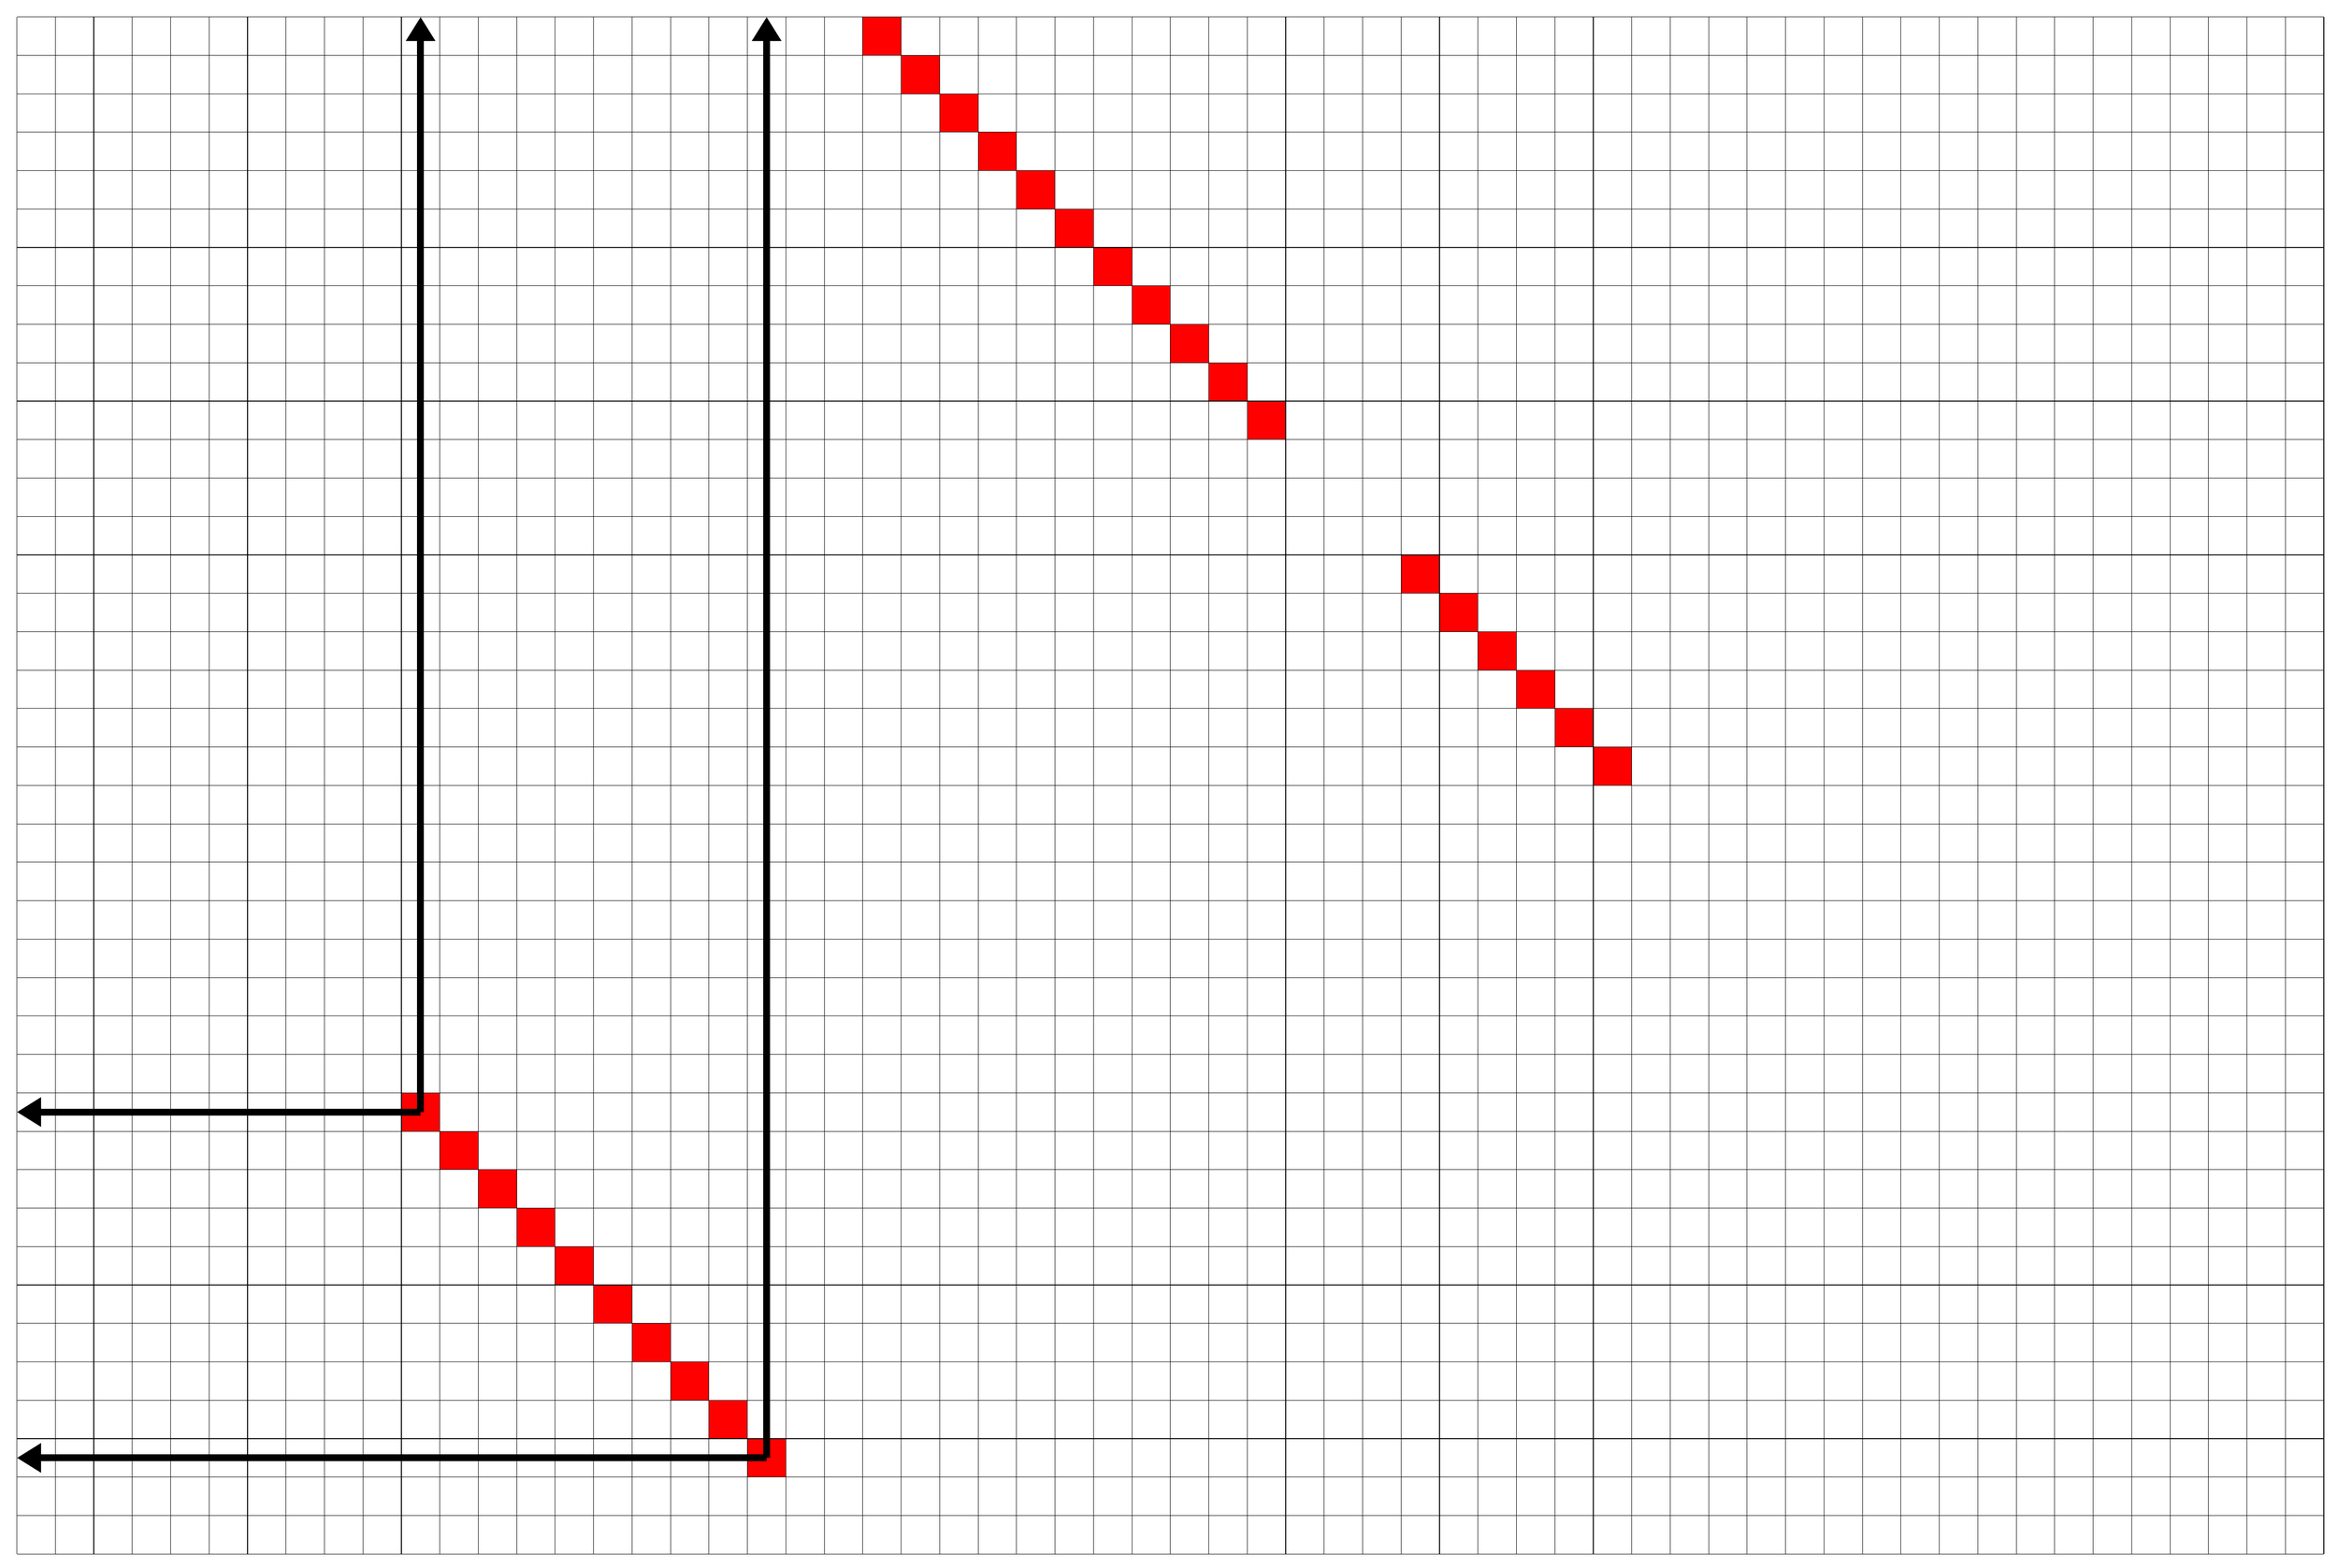
\begin{tikzpicture}[every node/.style={minimum size=1cm-\pgflinewidth, outer sep=0pt, fill=green}]
	\DrawDiagonal{-8}{20}{10}
	\DrawDiagonal{6}{6}{5}
	\DrawDiagonal{-20}{-8}{9}
	\path [draw, line width=5pt, ->, >=Triangle] (-19.5,-8.5) -- (-19.5, \yMax);
	\path [draw, line width=5pt, ->, >=Triangle] (-19.5,-8.5) -- (\xMin, -8.5);
	\path [draw, line width=5pt, ->, >=Triangle] (-10.5,-17.5) -- (-10.5, \yMax);
	\path [draw, line width=5pt, ->, >=Triangle] (-10.5,-17.5) -- (\xMin, -17.5);
	\draw[step=1cm,color=black](\xMin,\yMin) grid (\xMax, \yMax);
	\end{tikzpicture}
\end{document}